
\chapter{Outils existants pour le traitement des flux de donn\'ees}
\label{outils_connus}

\gt{Un nouveau chapitre doit (habituellement) avoir quelques
paragraphes d'introduction, qui indiquent ce dont va traiter le
chapitre.  Ce peut \^etre quelques paragraphes pr\'esent\'es
directement, sans num\'ero de section.  Ce peut aussi \^etre, quand il
y a plusieurs \'el\'ements \`a pr\'esenter, une section .1 appel\'ee
Introduction.  Ici, quelques paragraphes, sans section, devraient
\^etre suffisants.}


\ic{J'ai ajout\'e une petite introduction pour ce chapitre.}



\gt{Concernant les citations~: il y a deux macros que tu peux
utiliser: cite vs.\ citep: tu dois utiliser cite si tu veux que les
noms d'auteurs apparaissent comme sujet dans une phrase (avec
l'ann\'ee entre parenth\`eses)~; tu dois utiliser citep si tu veux que
la r\'ef\'erence soit compl\`etement entre parenth\`eses. Voir les
exemples ci-haut et ci-bas.}


La programmation parall\`ele devient de plus en plus une n\'ecessit\'e avec l'apparition des architectures multicœurs. Il y a quelques ann\'ees, la principale fa\c{c}on d'ex\'ecuter un programme plus rapidement \'etait d'augmenter la vitesse d'horloge du processeur. De nos jours, la vitesse d'horloge a atteint ses limites et la performance d'un programme ne peut souvent \^etre am\'elior\'ee que si on l'ex\'ecute en parall\`ele. 

Le paradigme de programmation parall\`ele par flux de donn\'ees offre une approche prometteuse pour la programmation de syst\`emes multicœurs. Les flux de donn\'ees sont utilis\'es dans plusieurs domaines, par exemple, traitement d'images, de donn\'ees r\'eseau, de donn\'ees et transactions boursi\`eres, de donn\'ees de trafic routier, etc.



Il existe de nombreux syst\`emes de traitement de flux de donn\'ees. La conception, le mod\`ele et l'architecture de ces syst\`emes diff\`erent, de sorte qu'ils poss\`edent des fonctionnalit\'es et des performances diff\'erentes. Ce chapitre pr\'esente un aper\c{c}u de trois syst\`emes de traitement de flux de donn\'ees~: \TT{Apach Spark}, les \TT{Stream} de Java~8 et \TT{FastFlow}.  Ce sont trois parmi les nombreux syst\`emes actuellement disponibles, que nous avons choisis de pr\'esenter parce qu'ils ont servi d'inspiration et de base au syst\`eme que nous avons d\'evelopp\'e, \ppff, pr\'esent\'e aux chapitres~\ref{description.chap} et~\ref{implementation.chap}.


\section{Apach Spark}

\TT{Apache Spark} \citep{apachSpark} est un outil de traitement par lots qui a aussi des capacit\'es de traitement des flux de donn\'ees. Conçu initialement pour r\'esoudre certaines problématiques de l'approche MapReduce (par ex., Hadoop \citep{white2012hadoop}), Spark se concentre principalement sur l'acc\'el\'eration du traitement des donn\'ees en gardant en m\'emoire les donn\'ees de travail.

Alors que le traitement en m\'emoire contribue consid\'erablement \`a la vitesse, Spark est \'egalement rapide avec le traitement de donn\'ees sur disques en raison de l'optimisation qui peut \^etre r\'ealis\'ee en analysant l'ensemble complet des t\^aches \`a l'avance. Ceci peut \^etre r\'ealis\'e en cr\'eant des graphes acycliques dirig\'es (DAG) qui repr\'esentent toutes les op\'erations qui doivent \^etre ex\'ecut\'ees, les donn\'ees \`a \^etre utilis\'ees, ainsi que les relations entre elles. \`A l'aide de ce m\'ecanisme, le processeur a la capacit\'e de coordonner le travail intelligemment.

Afin d'implémenter le traitement de donn\'ees, Spark utilise le mod\`ele appel\'e \TT{Resilient Distributed Datasets (RDD)} \citep{Salloum2016} qui g\`ere efficacement la m\'emoire. De plus, il impl\'emente le mod\`ele \TT{Discretized Streams} \citep{zaharia2013discretized} pour le traitement de flux.


\subsection{Resilient Distributed Dataset (RDD)}

\TT{RDD} est une abstraction de m\'emoire qui \'evite la r\'eplication de donn\'ees et minimise les recherches sur disque. Il permet aux applications de mettre en cache des donn\'ees \`a travers diff\'erentes \'etapes de traitement, ce qui acc\'el\`ere consid\'erablement la r\'eutilisation pour les donn\'ees futures. De plus, les RDD peuvent se souvenir des op\'erations utilis\'ees pour les construire. Lorsqu'une panne survient, ils peuvent reconstruire les donn\'ees avec une surcharge du r\'eseau minimale.

Les \TT{RDD} sont conçus pour \^etre partitionn\'es. Chaque partition contient des enregistrements qui peuvent \^etre cr\'e\'es par op\'erations de transformations. Les transformations incluent les opérations \TT{map}, \TT{filter}, \TT{groupBy} et \TT{join}.

Les \TT{RDD} peuvent \^etre cr\'e\'es via d'autres \TT{RDD} existants. Ce m\'ecanisme permet la reconstruction des partitions perdues, car chaque \TT{RDD} dispose d'informations suffisantes sur la reconstruction \`a partir d'autres \TT{RDD}. Lorsqu'il y a une demande de mise en cache d'un \TT{RDD}, Spark stocke ses partitions par d\'efaut en m\'emoire. Cependant, des partitions peuvent \^etre stock\'ees sur des disques lorsque la m\'emoire est insuffisante. 


\subsection{Discretized Streams}

\TT{Spark} traite un flux de donn\'ee par l'implémentation du mod\`ele \TT{Discretized Streams (D-streams)}. \TT{D-stream} repr\'esentent les flux de donn\'ees pris en entr\'ee pour le traitement. Il d\'ecompose un flux de donn\'ees en une s\'erie de petits lots dans de petits intervalles de temps appel\'es \TT{micro-batches}. Chaque \TT{micro-batch} stocke ses donn\'ees dans des \TT{DDR}. Ensuite, le \TT{micro-batch} est trait\'e et ses r\'esultats sont stock\'es dans des \TT{DDR} interm\'ediaires.


\section{Java 8 et ses \TT{Stream}s}

La version 8 de Java, qui a introduit les \TT{Stream}s, a chang\'e la façon dont les d\'eveloppeurs peuvent traiter, tant de fa\c{c}on s\'equentielle que parall\`ele, les collections de donn\'ees. La manipulation des \TT{Stream}s ressemble \`a un langage de requ\^ete de base de donn\'ees. Au lieu de parcourir explicitement les donn\'ees \`a l'aide de boucles (\TT{for}), les d\'eveloppeurs sp\'ecifient simplement des suites d'op\'erations \`a effectuer sur les \'el\'ements d'une collection. \cite{urma2014java} fournissent une description d\'etaill\'ee des nouveaux concepts introduits dans \TT{Java~8}. Les \TT{Stream}s et les \emph{expressions-lambdas} sont les fonctionnalit\'es les plus remarquables ajout\'ees dans l'API \citep{javaStreamAPI}. Ils sont con\c{c}us pour traiter les collections de donn\'ees de mani\`ere simple et efficace. Cette section d\'ecrit quelques-uns des concepts de \TT{Java~8}.


\subsection{Expressions lambda}


\gt{Bon, apr\`es avoir jet\'e un coup d'oeil \`a la documentation de
lstlisting et \`a des m\'emoires et th\`eses r\'ecentes, je constate
qu'il est pr\'ef\'erable {\bf de ne pas utiliser la macro Listing},
mais d'utiliser plut\^ot les divers arguments de l'environnement
lstlisting.  Ceci permettra une pr\'esentation plus uniforme des
diff\'erents listings et, surtout, une num\'erotation correcte (et
uniforme), dans le vrai style requis~: listing 1.1, 1.2, etc. pour le
chapitre 1; listing 2.2, 2.2, etc pour la chapitre 2 --- donc comme
pour les figures.}


\begin{lstlisting}[
label={exLambda},
language=java,
gobble=4,
caption={[Un exemple d'une expression lambda qui re\c{c}oit deux valeurs de type entier en argument.]Un exemple d'une expression lambda qui re\c{c}oit deux valeurs de type entier en argument, affect\'ee \`a la variable \TT{a}. Un appel est ensuite effectu\'ee et le r\'esultat est affect\'e \`a la variable \TT{result}.},
frame=single,
float]
    interface Addable { int add (int x, int y); }
    
    int y = 2;
    int x = 3;
    
    // Affectation de l'expression lambda a une variable.
    Addable a = (int w, int z) -> { return w + z; };

    // Appel de l'expression lambda.
    int result = a.add(x, y);    
\end{lstlisting}



Une \emph{expression lambda} ---  appel\'ee aussi \emph{fonction anonyme} --- est un bloc de code avec des param\`etres qui peut \^etre d\'efini, comme n'importe quelle valeur, puis qui peut \^etre ex\'ecut\'e ult\'erieurement. Par exemple, la fonction anonyme du listing~\ref{exLambda}, qui re\c{c}oit deux valeurs de type entier en argument et renvoie leur somme, est affect\'ee \`a la variable \TT{a}. Un appel \`a la m\'ethode \TT{add} --- de l'interface \TT{Addable} --- est ensuite effectu\'ee avec des arguments effectifs (\TT{x} et \TT{y}).


\begin{lstlisting}[
label={lambdaAsFonctionalInterface},
language=java,
gobble=4,
caption={Remplacement d'une classe anonyme avec une expression lambda.},
frame=single,
float]
    // Specification d'un thread avec une classe interne anonyme.
	Thread th = new Thread( new Runnable() {
		public void run() {
          ...
		}
	});

    // Specification d'un thread avec une expression lambda.
	Thread th = new Thread( () -> {
         ...
	});
\end{lstlisting}


\gt{Citation trop r\'ecente pour Haskell, qui ne montre pas que c'est quand m\^eme un ancien langage. Je l'ai remplac\'e. Idem pour Lisp.}

Le concept d'expression lambda n'est pas nouveau. Il est utilis\'e depuis longtemps dans les langages de programmation fonctionnelle tels que \TT{Lisp}~\citep{Steele84} ou \TT{Haskell}~\citep{HudakWad90,hutton2016programming}.
%
Les expressions lambda rendent le code plus concis et, dans le cas de \TT{Java}, l'\'etendent avec des concepts de langages de programmation fonctionnelle. 

Plus sp\'ecifiquement, en Java, ce concept est li\'e \`a celui d'interface fonctionnelle. Une expression lambda peut \^etre sp\'ecifi\'ee \`a la place d'une valeur dont le type est une interface fonctionnelle. Par exemple, le listing~\ref{lambdaAsFonctionalInterface} montre un exemple o\`u un \TT{thread}, d\'eclar\'e en utilisant la syntaxe de classe anonyme, peut \^etre \'ecrit plus facilement avec une expression lambda.

Dans une expression lambda, lors de la compilation, les types des arguments peuvent \^etre automatiquement d\'etermin\'es par le compilateur. Cette fonctionnalit\'e permet de passer des m\'ethodes comme arguments plut\^ot que de construire un objet d'une classe sp\'ecifique. Ceci permet \`a un programmeur de construire facilement des pipelines d'op\'erations fonctionnelles.


\subsection{It\'erations}


\begin{lstlisting}[
label={comparisonInternVsExtern},
language=java,
gobble=4,
caption={[Comparaison entre une it\'eration externe et interne.]Comparaison entre une it\'eration externe et interne~: dans le cas de l'it\'eration externe, le d\'eveloppeur d\'efinit une boucle explicite pour traiter les divers \'el\'ements de la collection.  Le traitement appliqu\'e \`a chaque \'el\'ement consiste \`a convertir la cha\^ine en lettres majuscules si elle d\'ebute par la lettre <<J>>. Le m\^eme traitement est appliqu\'e dans le cas de l'it\'eration interne. Par contre, dans ce cas, c'est le \TT{stream} qui contr\^ole le processus d'it\'eration~; l'usager  indique simplement les diverses op\'erations \`a effectuer, en les chainant les unes \`a la suite des autres.},
frame=single,
float]
    List<String> myList =
            Arrays.asList("Tom", "John", "Harry", "Jonathan");

    // Iteration externe avec ajout explicite (style imperatif).
    List<String> resultExtern = new ArrayList<String>();
    for (String s: myList){
        if (s.startsWith("J")) // Selection
           // Transformation et ajout dans le resultat.
           resultExtern.add(s.toUpperCase()); 
    }
        
    // Iteration interne avec pipeline d'operations (style fonctionnel).
    List<String> resultIntern = 
        myList
        .stream()
        .filter(s -> s.startsWith("J")) // Selection.
        .map(String::toUpperCase)       // Transformation.
        .collect(Collectors.toList());  // Collecte du resultat.
\end{lstlisting}


Une it\'eration est le processus qui consiste \`a traverser une s\'equence d'\'el\'ements pour traiter chacun d'entre eux. Avec les \TT{Stream}s \TT{Java}, une it\'eration peut \^etre ex\'ecut\'ee de deux mani\`eres : par une it\'eration \emph{externe} ou \emph{interne}. Une it\'eration est dite \emph{externe} lorsque le d\'eveloppeur contr\^ole la travers\'ee des \'el\'ements.  L'acc\`es et l'op\'eration sur chaque \'el\'ement de la collection sont d\'efinis par l'utilisateur. Par contre, une it\'eration est dite \emph{interne} lorsque la s\'equence contr\^ole elle-m\^eme tous les d\'etails du processus d'it\'eration. L'utilisateur fournit uniquement les op\'erations permettant de traiter les \'el\'ements, sans se soucier de la mani\`ere dont les \'el\'ements sont acc\'ed\'es et fournis. Le listing~\ref{comparisonInternVsExtern} montre un exemple d’une comparaison entre une itération externe et interne. 

L'approche interne est attrayante pour les opportunit\'es qu'elle offre aux compilateurs, notamment l'optimisation de l'exécution et les m\'ecanismes de nettoyage n\'ecessaires en arri\`ere-plan. Un autre avantage des it\'erations internes est l'efficacit\'e~: le traitement de donn\'ees peut \^etre plus efficace car il peut \^etre r\'eparti en parall\`ele parmi les cœurs de la machine.


\begin{figure}[H]
\centering
     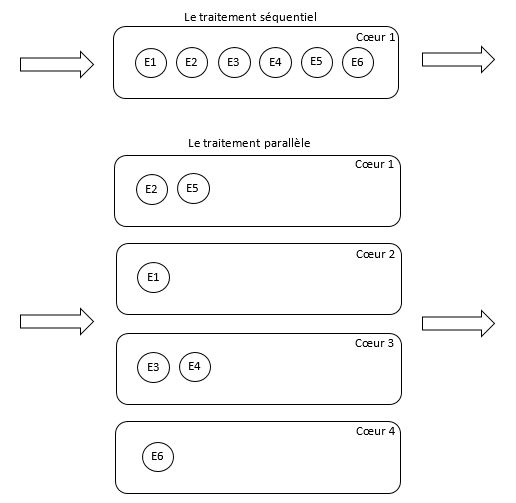
\includegraphics[width=1.0\textwidth]{Figures/ComparisonSequentialVsParallel.jpg}
      \caption[La comparaison entre le traitement s\'equentiel et parall\`ele.]{La comparaison entre le traitement s\'equentiel et parall\`ele. Les six \'el\'ements du flux, E1 \ldots E6, sont r\'epartis en quatre sous-flux. Chaque sous-flux est trait\'e avec l'un de quatre cœurs disponibles. Les r\'esultats sont combin\'es apr\`es le traitement.}
       \label{ComparisonSequentialVsParallel.fig}
\end{figure}


Lorsqu'un flux s'ex\'ecute en parall\`ele, Java partitionne le flux en plusieurs sous-flux. Les op\'erations parcourent et traitent ces sous-flux en parall\`ele, puis combinent les r\'esultats. La figure~\ref{ComparisonSequentialVsParallel.fig} montre la comparaison entre  un traitement s\'equentiel et un traitement parall\`ele, dans cet exemple avec quatre c\oe{}urs. Les \'el\'ements du flux sont partitionn\'es en sous-flux et chaque sous-flux r\'esultant est trait\'e avec l'un de quatre cœurs disponibles.  



\subsection{Flux}


\begin{lstlisting}[
label={findFirst},
language=java,
gobble=2,
caption={Optimisation du traitement d'un flux en utilisant la technique d'\'evaluation court-circuit\'ee.},
frame=single,
float]
	List<Employee> employees;
	Optional<Employee> employee = employees.findFirst();
\end{lstlisting}


Un flux est d\'efini comme une s\'equence immuable d'\'el\'ements fournissant une vari\'et\'e d'op\'erateurs et de m\'ethodes permettant de traiter une collection de donn\'ees. Le flux prend en charge les op\'erations d'agr\'egation \citep{javaStreamAggregate} s\'equentielles et parall\`eles sans se soucier de la mani\`ere dont les \'el\'ements sont stock\'es ou accessibles. Pour effectuer un traitement, les op\'erations de flux sont compos\'ees dans un \TT{pipeline}. Un \TT{pipeline} est compos\'e d'une source, de z\'ero ou plusieurs op\'erations interm\'ediaires et d'une op\'eration terminale. Une source peut \^etre constitu\'ee d'une collection ou de tout objet impl\'ementant l'interface qui d\'efinit le m\'ecanisme permettant d'extraire les donn\'ees de la source. 
Les op\'erations sur les flux adoptent un m\'ecanisme d'\'evaluation paresseuse. L'\'evaluation paresseuse est une m\'ethode d'optimisation du traitement qui retarde l'\'etape du calcul jusqu'\`a ce qu'il soit nécessaire. En \TT{Java}, le traitement sur les \'el\'ements du flux est r\'ealis\'e seulement \`a l'activation de l'op\'eration finale et les \'el\'ements source ne sont consomm\'es qu'au besoin. Cela permet au compilateur d'optimiser le traitement des donn\'ees dans le \TT{pipeline}.
Une autre technique d'optimisation utilis\'ee par \TT{Java} est l'\'evaluation court-circuit\'ee (\emph{short-circuiting} en anglais). Dans un flux, seuls les \'el\'ements n\'ecessaires sont consomm\'es. Par exemple, dans le listing~\ref{findFirst}, l'opérateur \TT{findFirst} retourne le premier employ\'e trouv\'e dans une liste d'employ\'es~; les \'el\'ements restants du flux sont ignor\'es.


L'un des principaux avantages des flux est qu'ils peuvent \^etre \'evalu\'es soit de fa\c{c}on s\'equentielle, soit en parall\`ele. L'\'evaluation s\'equentielle est r\'ealis\'ee en ex\'ecutant toutes les op\'erations en \TT{pipeline} sur chaque \'el\'ement du flux. Lorsqu'un flux est \'evalu\'e en parall\`ele, il utilise un type sp\'ecial d'it\'erateur appel\'e \TT{Spliterator}. Ce dernier partitionne le flux de mani\`ere r\'ecursive en se divisant lui-m\^eme pour cr\'eer des flux enfants. Ce m\'ecanisme permet aux \emph{threads} de traverser plusieurs flux en parall\`ele. Les \emph{threads} sont g\'er\'es par un groupe de \emph{threads} de type \TT{fork/join}.


\subsection{\emph{Threads} de type Fork/join}

Introduit en \TT{Java~7}, le \emph{framework} \TT{fork/join} permet aux d\'eveloppeurs de sp\'ecifier des t\^aches pouvant \^etre subdivis\'ees et ex\'ecut\'ees en parall\`ele sur des machines multicœurs. Il est bas\'e sur deux op\'erations : \TT{fork} et \TT{join}. L'op\'eration \TT{fork} a pour r\^ole de diviser une t\^ache en plus petites sous-t\^aches ind\'ependantes, et ce  r\'ecursivement jusqu'\`a ce qu'elles soient assez simples pour \^etre ex\'ecut\'ees de mani\`ere ind\'ependante et asynchrone. L'op\'eration \TT{join} a pour r\^ole de fusionner les r\'esultats de toutes les sous-t\^aches de mani\`ere r\'ecursive en un seul r\'esultat.
Les sous-t\^aches obtenues par l'op\'eration \TT{fork} sont soumises \`a un \TT{ForkJoinPool}. Ce dernier est composé d'un ensemble de travailleurs. Le nombre de travailleurs dans un \TT{ForkJoinPool} est g\'en\'eralement limit\'e par le nombre de cœurs de la machine. Chaque travailleur peut ex\'ecuter une t\^ache \`a la fois. Les t\^aches en attente d'ex\'ecution sont stock\'ees dans une file appartenant \`a un travailleur. Une t\^ache en cours d'ex\'ecution peut g\'en\'erer de nouvelles t\^aches, qui sont ensuite mises en file  pour une ex\'ecution ult\'erieure. Lorsqu'un travailleur a termin\'e l'ex\'ecution d'une t\^ache, il essaie de prendre une t\^ache des files des autres travailleurs \`a l'aide d'un algorithme de vol de travail (\emph{work stealing algorithm} en anglais). Cet algorithme permet un \'equilibrage efficace de la charge de travail entre les divers travailleurs.


\subsection{Un exemple~: \TT{wordCount}}


\begin{lstlisting}[
basicstyle=\footnotesize\tt,
label={wordCountJava},
language=java,
caption={Le code source Java~8 d'une application de d\'ecompte du nombre d'occurrences des mots.},
frame=single,
escapechar=\#,
float]
public static void main(String[] args) throws IOException {
  String text = 
    "Lorem ipsum dolor sit amet, consectetur \n" +
    " adipiscing elit. Lorem ipsum dolor sit amet, consectetur \n" +
    " adipiscing elit. Lorem ipsum dolor sit amet.";
  
  ArrayList<String> lines = 
	new ArrayList<String>(Arrays.asList(text.split("\\n")));
	
  List<Map.Entry<String,Integer>> wordsCount = 
    lines
    .stream()
    .parallel()
    .flatMap(line->Arrays.stream(line.trim().split(" ")))
    .map(word->word.replaceAll("[^a-zA-Z]", "").toLowerCase())
    .filter(word->word.length() > 0)
    .map(word->new SimpleEntry<>(word, 1))
    .collect(toMap(e->e.getKey(), e->e.getValue(), (v1,v2)->v1+v2))
    .entrySet()
    .stream()
    .collect(Collectors.toList());   	
  
  wordsCount.forEach( x -> 
    System.out.println("'" + x.getKey() + 
                             "' => " + x.getValue()) );
}
#\hrule#

#\underline{R\'esultat de l'ex\'ecution:}#
  'dolor' => 3
  'lorem' => 3
  'amet' => 3
  'adipiscing' => 2
  'ipsum' => 3
  'elit' => 2
  'consectetur' => 2
  'sit' => 3
\end{lstlisting}


Afin d'illustrer le mod\`ele de programmation avec les \TT{Stream}s de \TT{Java~8}, le listing~\ref{wordCountJava} montre le code source d'une application de d\'ecompte des mots --- plus pr\'ecis\'ement, l'application compte le nombre d'occurrences des divers mots dans un fichier texte. Une telle application est compos\'ee de plusieurs op\'erations cha\^in\'ees les unes \`a la suite des autres :


\begin{itemize}
	\item La premi\`ere op\'eration, \TT{Files.lines}, renvoie un flux s\'equentiel de lignes \`a partir du fichier. Le fichier est rep\'er\'e par le param\`etre \TT{inputFile} fourni en argument.

	\item La deuxi\`eme op\'eration, \TT{parallel}, marque le flux en tant que flux parall\`ele. Cette op\'eration permet ainsi de partitionner et d'ex\'ecuter le \TT{pipeline} en parall\`ele.

	\item L'op\'eration \TT{flatMap} divise chaque ligne en mots qui sont ensuite transmis en aval sous forme d'\'el\'ements de donn\'ees individuels.
	
	\item L'op\'eration \TT{map} supprime tous les caract\`eres qui ne sont pas des lettres puis transforme les lettres majuscules du mot en lettres minuscules.
	
	\item L'op\'eration \TT{filter} s\'electionne dans le flux seulement les mots qui ne sont pas vides.
	
	\item La deuxi\`eme op\'eration \TT{map} dans le pipeline cr\'ee une paire, de type \TT{Entry}, avec la cl\'e repr\'esent\'ee par le mot et une valeur associ\'ee \'egale \`a 1.
	
	\item L'op\'eration \TT{collect} collecte les \'el\'ements dans un \TT{Map} et additionne le nombre d'occurrences de chacun des mots \`a l'aide de l'expression lambda.
	
	\item L'op\'eration \TT{entrySet} renvoie un flux de type cl\'e--valeur. La cl\'e est le mot et la valeur est son nombre d'occurrences dans le fichier.

	\item L'op\'eration \TT{stream} cr\'ee un nouveau flux de donn\'ees \`a partir de l'ensemble de paires.
	
	\item Finalement, la derni\`ere op\'eration, \TT{collect}, combine tous les \'el\'ements dans une liste.
	
	
\end{itemize}


\section{FastFlow}

\TT{FastFlow} est une biblioth\`eque \TT{C++} qui, \`a la base, offre un ensemble de m\'ecanismes de bas niveau pour supporter les flux de donn\'ees, s'ex\'ecutant sur des machines multicœurs avec m\'emoire partag\'ee. La facilit\'e de d\'eveloppement avec \TT{FastFlow} est rendue possible en utilisant un ensemble de \emph{squelettes algorithmiques} offerts par la biblioth\`eque. Son efficacit\'e provient principalement de la mise en œuvre optimis\'ee de m\'ecanismes de communication de bas niveau et de sa conception en couches. Les squelettes algorithmiques offerts par \TT{FastFlow} peuvent \^etre utilis\'es pour exprimer les mod\`eles les plus courants de parall\'elisme. Ces squelettes algorithmiques peuvent \^etre imbriqu\'es pour cr\'eer des mod\`eles hi\'erarchiques de parall\'elisme plus complexes.

\TT{FastFlow} a \'et\'e conçue selon plusieurs principes: conception en couches, efficacit\'e des communications et synchronisation, et support pour le parall\'elisme de flux.

\subsection{Conception en couches}


\TT{FastFlow} a \'et\'e conçue sous la forme d'une pile de couches pour permettre d'impl\'ementer des m\'ecanismes d'abstraction et d'optimisation \`a plusieurs niveaux. La figure~\ref{FastFlowLayers.fig} montre les trois principales couches: \emph{High-level patterns}, \emph{Core patterns} et \emph{Building blocks}. 

Le niveau le plus bas de la pile, \emph{Building blocks}, g\`ere les communications asynchrones entre les canaux de communication et g\`ere le cycle de vie des flux. Plus pr\'ecis\'ement, cette couche offre des services pour les couches sup\'erieures. Elle g\`ere les queues, les processeurs et les fils d'ex\'ecutions (\emph{threads}).

Au-dessus de la couche \emph{Building blocks} se trouve la couche \emph{Core patterns}, qui fournit des squelettes (gabarits) pour mod\'eliser le parall\'elisme de flux. Les trois mod\`eles fournis dans cette couche sont \emph{task-farm}, \emph{pipeline} et \emph{feedback}, qui permettent de construire des flux parall\`eles. 

Au sommet de la pile se trouve la couche \emph{High-level patterns}, qui permet d'exprimer le parall\'elisme de plus haut niveau. Elle fournit plusieurs m\'ethodes qui couvrent les paradigmes de programmation parall\`eles les plus courants : parall\'elisme de flux, parall\'elisme de donn\'ees et  parall\'elisme de t\^aches. 

\begin{figure}[ht]
\centering
     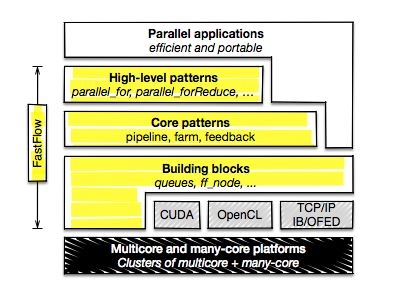
\includegraphics[width=1.0\textwidth]{Figures/FastFlowLayers.jpg}
      \caption[Les couches de \TT{FastFlow}.]{Les couches de \TT{FastFlow} --- figure tir\'ee de~\cite{Torquati15}.}
       \label{FastFlowLayers.fig}
\end{figure}

\subsection{Efficacit\'e}

L'id\'ee de \TT{FastFlow} est de fournir au programmeur des files (\emph{queues}) \emph{MP (Multiple Producer)} et des files \emph{MC (Multiple Consumer)} sans verrouillage, et ce afin de supporter des acc\`es rapides aux flux de donn\'ees. G\'en\'eralement, dans les applications de flux de donn\'ees, les canaux de communication sont impl\'ementés via des files de type \emph{MPMC (Multiple Producer/Multiple Consumer)}. Dans ce modèle, les acteurs se synchronisent simultanément pour acc\'eder aux donn\'ees. Ces synchronisations sont habituellement support\'ees par une ou plusieurs op\'erations atomiques --- par exemple, \TT{Compare-And-Swap} --- qui se comportent comme des barri\`eres de m\'emoire, ce qui augmente le co\^ut des synchronisations. Afin d'\'eviter les barri\`eres de m\'emoire, \TT{FastFlow} b\^atit les files \emph{MPMC} en assemblant des files, sans barri\`ere de m\'emoire, de type \emph{SPSC (Single Producer/Single Consumer)}. Dans ce mod\`ele, des files d’ex\'ecution regroupent ou \'emettent les donn\'ees des files d'entr\'ee vers les files de sortie. Selon son r\^ole, une file d'ex\'ecution peut \^etre un \TT{Emitter} ou un \TT{Collector}. Alors que l'\TT{Emitter} lit les donn\'ees, le \TT{Collector} \'ecrit sur une ou plusieurs files de types \emph{SPSC}. Contrairement aux op\'erations atomiques, ce m\'ecanisme n\'ecessite seulement des copies de m\'emoire --- la performance offerte par cette solution d\'ecoule de la vitesse sup\'erieure de la copie par rapport \`a la barri\`ere de m\'emoire.


\subsection{Parall\'elisme de flux}

Dans \TT{FastFlow}, le parall\'elisme de flux est repr\'esent\'e par un flux de donn\'ees comportant une s\'erie d'\'etapes, s\'equentielles ou parall\`eles, appel\'ees \emph{stages}. Chaque \emph{stage} lit les donn\'ees \`a partir du flux d'entr\'ee, effectue des calculs et traitements, puis \'ecrit le r\'esultat sur le flux de sortie. Le calcul repr\'esente une s\'equence de transformations sur les donn\'ees. Le parall\'elisme est obtenu en ex\'ecutant chaque \emph{stage} simultan\'ement sur des \'el\'ements ind\'ependants ou sur des sous-s\'equences d'\'el\'ements. 

Dans \TT{FastFlow}, le parall\'elisme peut \^etre obtenu en exploitant directement les mod\`eles parall\`eles disponibles dans la couche \emph{Building blocks}. En particulier, cela peut \^etre r\'ealis\'e des deux fa\c{c}ons suivantes :

\begin{itemize}
\item en d\'efinissant des activit\'es concurrentes s\'equentielles en sous-classant la classe \TT{ff\_node}~;
 
\item en construisant des mod\`eles parall\`eles complexes en composant de mani\`ere hi\'erarchique des activit\'es concurrentes s\'equentielles, soit avec des \emph{pipelines} --- \TT{ff\_pipeline} --- ou des \emph{farms} --- \TT{ff\_farm}.
\end{itemize}

\subsubsection*{La classe \TT{ff\_node}}

Dans \TT{FastFlow}, \TT{ff\_node} est la classe de base pour un noeud de traitement. Elle fournit les m\'ecanismes appropri\'es pour d\'efinir des activit\'es s\'equentielles pour le traitement de données apparaissant sur un canal d'entr\'ee et fournissant les r\'esultats correspondants sur un canal de sortie. 

La classe \TT{ff\_node} d\'efinit plusieurs m\'ethodes, les trois plus importantes \'etant les suivantes :
\begin{lstlisting}[language=c++]
  class ff_node {
    ...
    virtual void* svc(void* task) = 0
    virtual int svc_init() { return 0; } 
    virtual void svc_end() {} 
    ...
  }
\end{lstlisting}

La premi\`ere m\'ethode (\TT{svc}, mn\'emonique <<service>>) est celle qui d\'efinit le comportement du nœud lors du traitement des \'el\'ements du flux d'entr\'ee. Les deux autres m\'ethodes sont automatiquement appel\'ees lorsque le traitement repr\'esent\'e par le nœud est d\'emarr\'e \TT{(svc\_init)} et juste avant qu'il soit termin\'e \TT{(svc\_end)}. Ces m\'ethodes virtuelles peuvent \^etre red\'efinies dans des sous-classes \TT{ff\_node} sp\'ecifi\'ees par le programmeur afin d'impl\'ementer le traitement, l'initialisation ou la finalisation du code.


\subsubsection*{La classe \TT{ff\_pipeline}}

Un \emph{pipeline} est utilis\'e pour mod\'eliser les traitements exprim\'es par des \emph{stages}. Il est repr\'esent\'e par la classe \TT{ff\_pipeline}. Un {pipeline} peut comporter plusieurs \emph{stages}, peut \^etre construit comme un pipeline \`a \emph{n} \emph{stages}, ou encore comme un {pipeline} de {pipelines}. Un \emph{stage} peut \^etre de type \TT{ff\_node} ou \TT{ff\_farm}.


\goodbreak

\subsubsection*{La classe \TT{ff\_farm}}
\label{farm.sect}

\begin{figure}[ht]
\centering

\gt{Quand une l\'egende (caption) est trop longue, avec plein
d'explications, il est pr\'ef\'erable de mettre une version plus
courte entre crochets~: c'est alors cette derni\`ere qui apparait dans
la table des mati\`eres, plut\^ot que le long (long) texte. (Et voir
aussi ci-haut comment on peut faire de m\^eme pour un lstlisting: avec
crochets aussi mais un peu diff\'erent.)}

     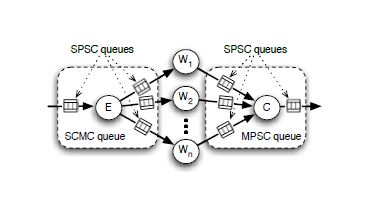
\includegraphics[width=1.0\textwidth]{Figures/FastFlowFarm.jpg}
      \caption[Les trois parties d'un \emph{farm} de \TT{FastFlow}.]{Un \emph{farm} de \TT{FastFlow} est compos\'e de trois parties~:  l'\TT{Emitter (E)}, le \emph{pool} de \TT{workers} (W1\ldots\ Wn) et le \TT{Collector (C)}. Les canaux de communication sont impl\'ement\'es en assemblant des files de types \emph{Simple Producer/Simple Consumer (SPSC)} --- figure tir\'ee de~\citep{aldinucci2010efficient}.}
       \label{FastFlowFarm.fig}
\end{figure}

Un \emph{farm} est bas\'e sur la r\'eplication d'une fonction. Dans \TT{FastFlow}, un \emph{farm} est repr\'esent\'e par un objet de la classe \TT{ff\_farm}. Comme le montre la figure~\ref{FastFlowFarm.fig}, un \emph{farm} est compos\'e de trois parties distinctes: un \TT{Emitter}, un  \emph{pool} de \TT{workers} et un \TT{Collector}. L'\TT{Emitter} est responsable de la r\'epartition des \'el\'ements du flux au \emph{pool} de \TT{workers}, lesquels traitent et produisent les donn\'ees de sortie; l'\TT{Emitter} distribue les \'el\'ements d'entr\'ee aux travailleurs selon une certaine politique d'ordonnancement afin d'\'equilibrer la charge des travailleurs. Les r\'esultats sont ensuite rassembl\'es par le \TT{Collector} dans un seul flux. Les communications entre \TT{Emitter} et \TT{Collector} se font via des canaux de communication sans barri\`eres de m\'emoire, tel que d\'ecrit pr\'ec\'edemment.


\subsection{Un exemple~: \TT{WordCount}}


\begin{lstlisting}[language=c++, 
caption={Le code source FastFlow d'une application de d\'ecompte du nombre d'occurrences des mots.},
label={wordcountFastFlow},
frame=single,
float,
numbers=left
]
 #define DEFAULT_INPUT_FILE "Words.txt"
 typedef std::vector<std::string> Words;
 
 struct linesFromFileStage: ff_node {
    std::string const &path;
    linesFromFileStage(std::string const &path): path(path){}
 
    void* svc(void* task) {
       std::ifstream file(path);
       std::string* line = new std::string;
       while (std::getline(file, *line)) {
           ff_send_out(line);
           line = new std::string;
       }
       return EOS;
    }
 };
 
 struct splitInWordsStage: ff_node {
    std::string delimiter = " ";
    void* svc(void* task) {
       std::string line = *((std::string*)task);
       Words* words = new Words();
       size_t start = 0, end = 0;
       do {
           end = line.find(delimiter, start);
           size_t len = end - start;
           words->push_back( line.substr(start, len) );
           start += len + delimiter.length();
       } while (end != std::string::npos);

       return words;
    }
 };
\end{lstlisting}
 
\begin{lstlisting}[language=c++, frame=single,float,numbers=left,firstnumber=35]
 struct flatStage: ff_node {
    std::string delimiter = " ";
    void* svc(void* task) {
        for (auto &elem: *(Words*)task) {
            ff_send_out(&elem);
        }
        return GO_ON;
    }
 };
 
 struct groupByKeyStage: ff_node {
    typedef std::unordered_map<std::string, int> CONTAINER;
    CONTAINER &container;
    groupByKeyStage(CONTAINER &container): container(container){}
    void* svc(void* task) {
       container[*((std::string*)task)] += 1;
       return GO_ON;
    }
 };
\end{lstlisting}
 
\begin{lstlisting}[language=c++, frame=single, float, numbers=left,firstnumber=54]
 int main(int argc, char *argv[]) {
     std::unordered_map<std::string, int> result;
     std::string inputFile = DEFAULT_INPUT_FILE;

     if (argc >= 2) { inputFile = argv[1]; } 

     linesFromFileStage linesFromFile(inputFile);
     splitInWordsStage splitInWords;
     flatStage flat;
     groupByKeyStage groupByKey(result);

     ff_pipeline ffp;
     ffp.add_stage(&linesFromFile);
     ffp.add_stage(&splitInWords);
     ffp.add_stage(&flat);
     ffp.add_stage(&groupByKey);

     if (ffp.run_and_wait_end() < 0) error("running pipe");
     return 0;
 }
\end{lstlisting}

Cette section pr\'esente un exemple d'un programme r\'ealis\'e en \TT{FastFlow}. Illustr\'e dans le listing~\ref{wordcountFastFlow}, ce programme compte le nombre d'occurrences des divers mots dans un fichier texte. 

Un {pipeline} de \TT{n} \TT{stages} distincts est cr\'e\'e en instanciant les \TT{n} diff\'erents \TT{stages}; ensuite leurs r\'ef\'erences sont transmises dans le bon ordre au {pipeline}. Dans l'exemple du listing~\ref{wordcountFastFlow}, les \TT{stages} sont repr\'esent\'es par les op\'erations du programme de d\'ecompte du nombre de mots --- lignes 66 \`a 69.  Les quatre op\'erations r\'ealisent les fonctions suivantes :

\begin{itemize}
    \item La premi\`ere op\'eration, \TT{linesFromFile}, renvoie un flux s\'equentiel de lignes \`a partir du fichier. Le fichier est identifi\'e par le param\`etre \TT{inputFile} fourni en argument.

    \item La deuxi\`eme op\'eration, \TT{splitInWords}, divise chaque ligne en mots qui sont ensuite transmis en aval sous forme d'une collection de mots.
    
    \item La troisi\`eme op\'eration, \TT{flat}, décompose la collection en mots individuels, lesquels sont ensuite transmis dans le flux en tant qu'éléments individuels de données.
    
    \item La derni\`ere op\'eration, \TT{groupByKey}, regroupe les mots similaires ensemble et ensuite compte le nombre d'occurrences de chaque mot.
    
\end{itemize}
